\documentclass[11pt,a4paper]{article}

% ================================================================ paquets
\usepackage[T1]{fontenc}
\usepackage[utf8]{inputenc}
\usepackage[french]{babel}
\usepackage{newtxtext,newtxmath}
\usepackage[margin=2.4cm]{geometry}
\usepackage{amsmath,amssymb}
\usepackage{graphicx}
\usepackage{booktabs}
\usepackage{adjustbox}
\usepackage{xcolor}
\usepackage[font=small,labelfont=bf]{caption}
\usepackage[numbers,sort&compress]{natbib}
\usepackage[colorlinks=true,linkcolor=violet,citecolor=blue!60!black,urlcolor=blue!60!black]{hyperref}
\usepackage{microtype}
\usepackage{fancyhdr}

% Présentation de type prépublication arXiv
\pagestyle{fancy}
\fancyhf{}
\renewcommand{\headrulewidth}{0.4pt}
\fancyhead[C]{\small\scshape Prépublication, \today}
\fancyfoot[C]{\thepage}
\fancypagestyle{plain}{\fancyhf{}\renewcommand{\headrulewidth}{0pt}\fancyfoot[C]{\thepage}}
\setlength{\headheight}{14pt}

\graphicspath{{figures/}}

% ================================================================ titre
\title{\bfseries Le bruit sur les étiquettes déplace le seuil, pas le classement~:\\
modèles classiques et incertitude évidentielle\\ pour la détection de la pneumonie avec des étiquettes incertaines}

\author{
  \begin{adjustbox}{max width=\textwidth}
  \begin{tabular}{@{}c@{\hspace{3em}}c@{}}
    FOFACK ALEMDJOU Henri Jo\"el\textsuperscript{*} & ELOUNDOU NGOUMA Thomas Christian \\
    {\small 22P231} & {\small 22P294} \\[6pt]
    WATON JEUTA Ivana & WAFO TEGUO Vitric Val\`ere \\
    {\small 24P763} & {\small 22P446} \\[6pt]
    ZUCHUON KOUGANG Nathanael Michel & AYISSI NGONO Odile Marie Ange \\
    {\small 22P218} & {\small 24P764}
  \end{tabular}
  \end{adjustbox}\\[10pt]
  \small Département de Génie Informatique\\
  \small École Nationale Supérieure Polytechnique de Yaoundé (ENSPY)\\
  \small Université de Yaoundé I, Cameroun\\[4pt]
  \small \textsuperscript{*}Auteur correspondant
}
\date{}

\begin{document}
\maketitle

\begin{abstract}
Les étiquettes des images médicales sont souvent incertaines, alors que les classifieurs classiques les traitent comme
exactes. Nous étudions ce décalage sur PneumoniaMNIST. Neuf modèles classiques, dont une régression logistique
implémentée de zéro et entraînée par montée de gradient stochastique, des arbres boostés et des SVM à noyau, sont réglés
sur la validation puis soumis à l'inversion de 0 à 40\,\% des étiquettes d'entraînement de la classe minoritaire~; un
CNN évidentiel est comparé à un CNN softmax identique. Trois constats émergent. D'abord, le bruit asymétrique déplace
surtout le seuil de décision~: la spécificité chute d'environ 0,6 à 0,2--0,3 tandis que l'AUC ROC reste entre 0,92 et
0,95. Ensuite, une régularisation plus forte dégrade systématiquement les résultats, alors que re-choisir le seuil sur un
petit ensemble propre maintient l'exactitude entre 0,85 et 0,89 jusqu'à 40\,\% de bruit. Enfin, le modèle évidentiel
égale l'exactitude du softmax et est mieux calibré sous bruit (erreur de calibration 0,13 contre 0,21 à 20\,\% de
bruit), mais son incertitude n'améliore pas de façon fiable la détection hors distribution. Tous les résultats sont
reproductibles à partir de notebooks publics et d'exécutions MLflow.
\end{abstract}

\noindent\textbf{Mots-clés~:} classification d'images médicales $\cdot$ bruit d'étiquetage $\cdot$ étiquettes
incertaines $\cdot$ apprentissage profond évidentiel $\cdot$ théorie de Dempster--Shafer $\cdot$ calibration $\cdot$
précision--rappel $\cdot$ MLOps

% ======================================================================
\section{Introduction}
% ======================================================================
Les classifieurs supervisés d'images médicales sont entraînés sur des étiquettes elles-mêmes incertaines. Les
radiologues divergent sur les cas ambigus, les étiquettes extraites automatiquement des comptes rendus héritent de leurs
formulations prudentes (CheXpert marque explicitement ces observations comme \emph{incertaines}~\cite{irvin2019chexpert}),
et les erreurs d'annotation sont inévitables à grande échelle~\cite{karimi2020deep}. Un modèle ajusté comme si ces
étiquettes étaient exactes peut mémoriser le bruit~\cite{zhang2017understanding} et, plus insidieusement, renvoie une
probabilité confiante pour toute entrée, y compris celles sur lesquelles il ne dispose d'aucune évidence.

L'apprentissage automatique classique offre deux réponses génériques au bruit d'étiquetage~: la \emph{régularisation}
(pénalité plus forte en régression logistique ou en SVM, arbres moins profonds, boosting plus lent) et une
\emph{évaluation} rigoureuse sur des métriques qui restent informatives en cas de déséquilibre des
classes~\cite{saito2015precision}. Aucune ne permet pourtant au modèle de dire «~je ne sais pas~». L'apprentissage
profond évidentiel (EDL)~\cite{sensoy2018evidential} le permet~: fondé sur la théorie de
Dempster--Shafer~\cite{dempster1967upper,shafer1976mathematical} et la logique subjective~\cite{josang2016subjective}, il
fait produire au réseau une distribution de Dirichlet dont la force totale mesure la quantité d'évidence, et transforme
le manque d'évidence en une masse d'incertitude explicite. L'incertitude évidentielle a été utilisée sur des
radiographies thoraciques pour rejeter les cas peu fiables et signaler des erreurs d'annotation
probables~\cite{ghesu2019quantifying,ghesu2021quantifying}.

Ce rapport étudie, sur un banc d'essai volontairement léger mais réaliste (PneumoniaMNIST~\cite{yang2023medmnist}),
jusqu'où vont les outils classiques de robustesse face à l'incertitude des étiquettes, et ce qu'apporte un modèle
évidentiel. Nos contributions sont les suivantes~:
\begin{enumerate}
  \item une évaluation complète, réglée sur la validation, de neuf classifieurs classiques, dont une régression
        logistique implémentée de zéro et entraînée par montée de gradient stochastique (SGA), avec des intervalles de
        confiance bootstrap et une étude contrôlée montrant pourquoi les courbes précision--rappel doivent remplacer les
        courbes ROC lorsque la maladie est rare~;
  \item une étude factorielle du bruit d'étiquetage (propre/bruité $\times$ référence/régularisé/recalibré, 0 à
        40\,\% d'étiquettes minoritaires inversées, graines répétées) montrant que le bruit asymétrique \emph{déplace
        surtout le seuil de décision} en laissant le classement presque intact, et qu'une régularisation plus forte
        n'aide pas~;
  \item une implémentation PyTorch d'un CNN évidentiel comparée à un CNN softmax identique, évaluée non seulement sur
        l'exactitude mais aussi sur l'utilité de l'incertitude~: renvoi des cas douteux, détection d'images hors
        distribution et repérage des étiquettes d'entraînement inversées~;
  \item une chaîne MLOps reproductible (suivi MLflow, registre de modèles) et des notebooks publics générant chaque
        nombre, table et figure de ce rapport.
\end{enumerate}

% ======================================================================
\section{Travaux connexes}
% ======================================================================
\paragraph{Classification classique et régularisation.}
La régression logistique entraînée par des méthodes de gradient stochastique~\cite{robbins1951stochastic,bottou2010large},
le Bayes naïf~\cite{domingos1997optimality}, les plus proches voisins~\cite{beyer1999nearest}, les arbres de
décision~\cite{breiman1984classification}, le boosting~\cite{freund1997decision,friedman2001greedy} et les machines à
vecteurs de support (à noyau)~\cite{cortes1995support,scholkopf2002learning} restent des références solides sur les
petits jeux de données médicaux. Leur capacité est contrôlée par une régularisation explicite~: la pénalité inverse
$C$, la profondeur et la taille des feuilles des arbres, ou le taux d'apprentissage et le nombre d'itérations du
boosting.

\paragraph{Apprentissage avec des étiquettes bruitées.}
Le bruit d'étiquetage a fait l'objet de nombreuses synthèses~\cite{frenay2014classification,song2022learning}, y compris
en imagerie médicale~\cite{karimi2020deep}. Les remèdes incluent la correction de la perte sous un modèle de bruit
connu~\cite{natarajan2013learning}, des pertes robustes au bruit~\cite{ghosh2017robust,zhang2018generalized} et
l'identification des exemples mal étiquetés, par exemple par l'apprentissage confiant~\cite{northcutt2021confident}. Les
réseaux profonds peuvent ajuster des étiquettes arbitraires~\cite{zhang2017understanding}~: leur comportement sous bruit
dépend donc fortement des choix d'entraînement.

\paragraph{Quantification de l'incertitude.}
Les approximations bayésiennes comme le dropout Monte-Carlo~\cite{gal2016dropout} et les ensembles
profonds~\cite{lakshminarayanan2017simple} estiment l'incertitude à partir de plusieurs passes avant. Les réseaux à
a priori~\cite{malinin2018prior} et l'EDL~\cite{sensoy2018evidential} prédisent au contraire les paramètres d'une
distribution de Dirichlet en une seule passe~; voir~\cite{ulmer2023prior} pour une synthèse. L'incertitude est
généralement évaluée par la calibration~\cite{guo2017calibration}, la détection des erreurs et des exemples hors
distribution (OOD)~\cite{hendrycks2017baseline}, et la prédiction sélective~\cite{geifman2017selective}. En radiographie
thoracique, Ghesu \emph{et al.}~\cite{ghesu2019quantifying,ghesu2021quantifying} ont montré que l'incertitude
évidentielle permet de rejeter les cas ambigus et d'identifier le bruit d'étiquetage.

% ======================================================================
\section{Méthodologie}
% ======================================================================
\subsection{Données et prétraitement}
PneumoniaMNIST~\cite{yang2023medmnist} contient des radiographies thoraciques pédiatriques~\cite{kermany2018identifying}
redimensionnées en $28\times28$ pixels en niveaux de gris, avec des partitions officielles disjointes par patient de
4\,708 (entraînement), 524 (validation) et 624 (test) images. La tâche est binaire~: $y=1$ (pneumonie, classe positive)
contre $y=0$ (normal). Les images normales forment la classe minoritaire (25,8\,\% de l'entraînement)~; la prévalence de
la pneumonie passe de 74,2\,\% (entraînement et validation) à 62,5\,\% (test), un décalage d'acquisition réaliste
(figure~\ref{fig:samples}). Pour les modèles classiques, chaque image est aplatie en $x\in[0,1]^{784}$ et standardisée
avec les statistiques d'entraînement. Le jeu ne comporte aucune valeur manquante~; un masque simulé de 5\,\% de pixels
manquants complètement au hasard, imputé dans le pipeline, n'a fait baisser l'exactitude de validation de la régression
logistique que de 0,958 à 0,952 (imputation par la moyenne). \textbf{Tous les hyperparamètres sont choisis sur la
partition de validation}~; la partition de test n'est utilisée qu'une fois, pour le rapport.

\subsection{Modèles classiques}
\paragraph{Régression logistique par SGA.} Nous maximisons la log-vraisemblance pénalisée $\ell_2$ avec des mises à jour
exemple par exemple
\begin{equation}
  \theta \leftarrow \theta + \alpha_t\big[(y_i - \sigma(\theta^\top x_i + b))\,x_i - \lambda\theta\big],\qquad
  \alpha_t = \frac{\alpha_0}{1+\kappa t},
\end{equation}
avec $\alpha_0=0{,}01$, $\lambda=0{,}01$, $\kappa=10^{-4}$ et 30 époques. Chaque mise à jour coûte $O(m)$ au lieu de
$O(nm)$ pour la montée de gradient par lot~; sur un problème synthétique de 200\,000 exemples, le SGA arrive à moins de
0,005 de la meilleure log-vraisemblance de validation après 0,69 passe sur les données, contre 34 passes pour la montée
de gradient par lot (figure~\ref{fig:sga}). L'extension multiclasse (softmax) atteint 67,7\,\% d'exactitude en test sur
OrganCMNIST (11 classes), au niveau du solveur multinomial de scikit-learn (67,4\,\%). La sortie sigmoïde se lit comme
$P(y=1\mid x)$, c'est-à-dire un modèle de log-cote dont nous vérifions la calibration par un diagramme de fiabilité
(figure~\ref{fig:logreg}). Nous reportons aussi la solution L-BFGS de scikit-learn~\cite{pedregosa2011scikit}
($C=10^{-3}$).

\paragraph{Autres modèles.} Bayes naïf gaussien, dont l'hypothèse d'indépendance conditionnelle est fortement violée par
les pixels voisins (corrélation $\approx 0{,}92$) mais qui s'entraîne en une seule passe $O(nm)$~; $K$ plus proches
voisins ($K=7$, distance euclidienne), qui se dégradent bien moins avec la dimension que ne le suggère la concentration
des distances sur des données uniformes, car les radiographies vivent sur une variété de faible dimension
(figure~\ref{fig:knn})~; CART avec l'impureté de Gini (profondeur 13, au moins 5 exemples par feuille), dont nous avons
vérifié que le temps d'apprentissage croît linéairement en $n$, $m$ et en profondeur (figure~\ref{fig:tree})~; AdaBoost
avec des arbres de profondeur 2 (186 itérations, taux d'apprentissage 0,5)~; gradient boosting par histogrammes
(54 itérations, 15 feuilles, taux d'apprentissage 0,1, $\ell_2=1$)~; un SVM linéaire à marge souple (perte charnière,
$C=3{,}2\times10^{-3}$)~; et un SVM à noyau RBF ($C=3$, $\gamma=10^{-3}$) choisi sur une grille de validation
$4\times4$. Le rôle de $C$ sur la marge et le nombre de vecteurs supports, ainsi que la projection implicite des
noyaux, sont illustrés par les figures~\ref{fig:svm} et~\ref{fig:kernel}.

\subsection{Modèle de bruit et variantes robustes}
Conformément à l'énoncé, l'incertitude des étiquettes est simulée en inversant une fraction $\rho$ des étiquettes
d'entraînement de la \emph{classe minoritaire} (normal $\to$ pneumonie), c'est-à-dire avec la transition conditionnelle
à la classe $P(\tilde y=1\mid y=0)=\rho$, $P(\tilde y=0\mid y=1)=0$. Nous utilisons $\rho=5\,\%$ (61 des 1\,214 images
normales, 10 tirages) et un balayage $\rho\in\{0,5,10,20,30,40\}\,\%$ (5 tirages). Les étiquettes de validation et de
test ne sont jamais corrompues. Les trois meilleurs modèles en validation au sein des familles citées par l'énoncé
(arbres boostés, SVM à noyau et régression logistique régularisée) sont ré-entraînés dans trois configurations~:
(i)~\emph{référence} (hyperparamètres choisis sur la validation)~;
(ii)~\emph{robuste}~: régularisation plus forte ($C/10$ pour les SVM et la régression logistique~; 7 feuilles, taux
d'apprentissage divisé par deux, $\ell_2=10$ et au moins 50 exemples par feuille pour le boosting)~;
(iii)~\emph{recalibrée}~: le modèle de référence dont le seuil de décision est re-choisi pour maximiser l'exactitude
équilibrée sur la validation propre (un petit ensemble de confiance, sans ré-estimation des paramètres).

\subsection{CNN évidentiel}
Les deux modèles profonds partagent le même CNN (trois blocs de convolution $3\times3$ avec normalisation par lot,
16/32/64 canaux, moyenne globale, dropout 0,3, couche linéaire~; 23\,650 paramètres) et la même recette d'entraînement
(Adam, taux d'apprentissage $10^{-3}$, décroissance des poids $10^{-4}$, lots de 128, 15 époques, 3 graines), implémentés
en PyTorch~\cite{paszke2019pytorch}~; seules la couche de sortie et la perte diffèrent. Le modèle \textbf{softmax} est
entraîné avec l'entropie croisée. Le modèle \textbf{évidentiel}~\cite{sensoy2018evidential} transforme les logits $z$ en
évidences positives $e_k=\mathrm{softplus}(z_k)$ et en paramètres de Dirichlet $\alpha_k=e_k+1$. Avec
$S=\sum_k\alpha_k$ et $K=2$ classes, la logique subjective~\cite{josang2016subjective} donne des masses de croyance
$b_k=e_k/S$ et une masse d'incertitude (d'ignorance) $u=K/S$ avec $\sum_k b_k+u=1$~; la probabilité attendue de la
classe est $\hat p_k=\alpha_k/S$. La perte est le risque bayésien de l'entropie croisée sous la Dirichlet, plus un terme
de Kullback--Leibler recuit qui retire l'évidence non justifiée par l'étiquette~:
\begin{equation}
  \mathcal L_i=\sum_{k}y_{ik}\big(\psi(S_i)-\psi(\alpha_{ik})\big)
  +\lambda_t\,\mathrm{KL}\!\left(\mathrm{Dir}(p\mid\tilde\alpha_i)\,\big\|\,\mathrm{Dir}(p\mid\mathbf 1)\right),\quad
  \tilde\alpha_i=y_i+(1-y_i)\odot\alpha_i,\quad \lambda_t=\min(1,t/10),
\end{equation}
où $\psi$ est la fonction digamma et $t$ l'époque. Contrairement à la sortie softmax, la Dirichlet peut exprimer
«~aucune évidence~» ($S\to K$, $u\to1$) indépendamment d'une «~évidence équilibrée~» ($\hat p\approx0{,}5$ avec $u$
faible).

\subsection{Protocole d'évaluation}
Nous rapportons l'exactitude, la précision, le rappel (sensibilité), la spécificité, le F1, l'AUC ROC et la précision
moyenne (AP, aire sous la courbe précision--rappel), avec des intervalles de confiance bootstrap à 95\,\% (1\,000
rééchantillonnages du test). La calibration est mesurée par l'erreur de calibration attendue (ECE, 15
intervalles)~\cite{guo2017calibration}. Les scores d'incertitude (entropie prédictive normalisée pour le softmax, $u$
pour l'EDL) sont évalués par l'AUROC pour (a)~séparer les prédictions erronées des prédictions correctes en test,
(b)~séparer le test de PneumoniaMNIST d'images hors distribution d'autres modalités (échographies BreastMNIST et scanners
OrganCMNIST~\cite{yang2023medmnist}) et (c)~retrouver les étiquettes d'entraînement inversées. Chaque exécution de
l'étude de bruit est suivie avec MLflow~\cite{zaharia2018accelerating} (hyperparamètres, métriques, modèle sérialisé avec
sa signature d'entrée), et le modèle final est versionné dans le registre de modèles MLflow.

% ======================================================================
\section{Expériences et résultats}
% ======================================================================
\subsection{Modèles classiques sur étiquettes propres}
La table~\ref{tab:clean} et la figure~\ref{fig:rocpr} résument les neuf modèles classiques entraînés sur des étiquettes
propres. Le SVM à noyau classe le mieux les patients (AUC ROC 0,947, AP 0,961), le SVM linéaire obtient la meilleure
exactitude et le meilleur F1 (0,864 et 0,900), et notre régression logistique SGA implémentée de zéro (exactitude 0,851,
AUC ROC 0,927) est au niveau de la solution L-BFGS. Les intervalles bootstrap à 95\,\% du F1 sont larges et se
recouvrent nettement (par exemple $[0{,}859~;~0{,}905]$ pour la régression logistique contre $[0{,}880~;~0{,}920]$ pour
le SVM linéaire)~: sur 624 images de test, les écarts entre les meilleurs modèles restent dans l'incertitude
d'échantillonnage. L'arbre seul est clairement le moins bon pour classer (AUC ROC 0,747), et le boosting corrige ce
défaut (0,931 pour AdaBoost, 0,938 pour le gradient boosting~; figure~\ref{fig:boosting}). Tous les modèles partagent
une faiblesse~: un rappel de 0,90 à 0,99 mais une spécificité de seulement 0,57 à 0,73. Les exactitudes de validation
étaient bien plus élevées (jusqu'à 0,973 pour le SVM RBF), car le seuil appris avec une prévalence de pneumonie de
74\,\% est trop agressif pour la prévalence de 62,5\,\% du test. Les frontières de décision sur une projection ACP en
2D (figure~\ref{fig:boundaries}) illustrent les biais inductifs~: une droite unique avec des probabilités variant
continûment pour la régression logistique, des escaliers alignés sur les axes avec des probabilités constantes par
morceaux pour l'arbre, et une frontière courbe et lisse pour le SVM RBF.

\begin{figure}[t]
  \centering
  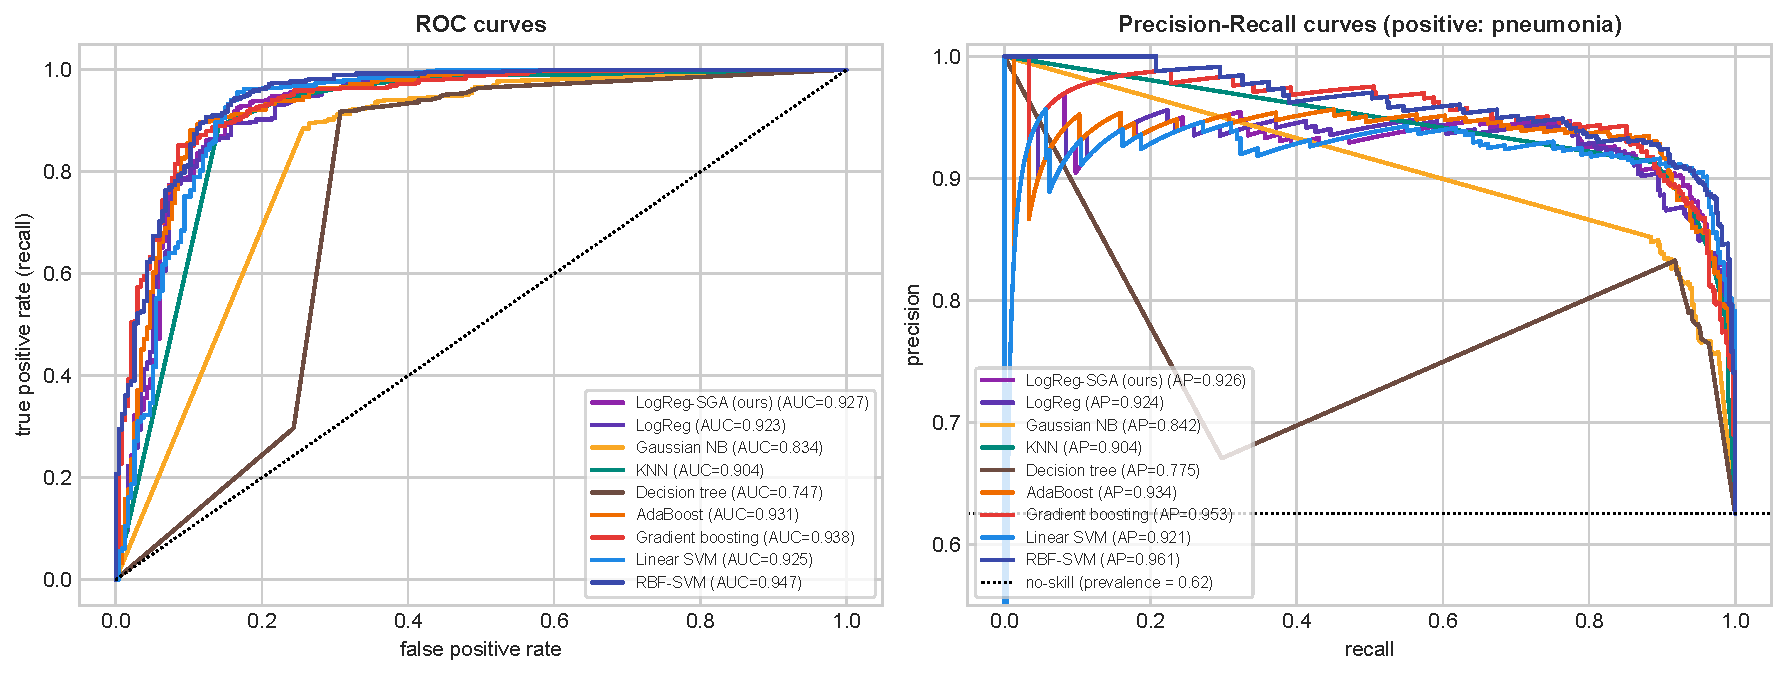
\includegraphics[width=\linewidth]{fig_roc_pr}
  \caption{Courbes ROC (gauche) et précision--rappel (droite) des modèles classiques sur le test propre (classe positive~:
           pneumonie). La ligne pointillée de la courbe PR est le niveau sans compétence, c'est-à-dire la prévalence.}
  \label{fig:rocpr}
\end{figure}

\begin{table}[t]
\centering
\small
\caption{Performances en test de tous les modèles classiques entraînés sur des étiquettes propres (classe positive~: pneumonie~; intervalle de confiance bootstrap à 95\,\% pour le F1-score). Meilleure valeur de chaque colonne en gras.}
\label{tab:clean}
\begin{adjustbox}{max width=\textwidth}
\begin{tabular}{lccccccc}
\toprule
Modèle & Acc. & Préc. & Rappel & Spéc. & F1 [IC 95\,\%] & ROC-AUC & AP \\
\midrule
LogReg-SGA (nôtre) & 0,851 & 0,814 & 0,987 & 0,624 & 0,892 [0,870~; 0,913] & 0,927 & 0,926 \\
LogReg & 0,837 & 0,800 & 0,985 & 0,590 & 0,883 [0,859~; 0,905] & 0,923 & 0,924 \\
Naive Bayes gaussien & 0,833 & \textbf{0,847} & 0,895 & \textbf{0,731} & 0,870 [0,846~; 0,894] & 0,834 & 0,842 \\
KNN & 0,830 & 0,793 & 0,985 & 0,573 & 0,879 [0,856~; 0,902] & 0,904 & 0,904 \\
Arbre de décision & 0,804 & 0,790 & 0,936 & 0,585 & 0,857 [0,831~; 0,881] & 0,747 & 0,775 \\
AdaBoost & 0,840 & 0,806 & 0,979 & 0,607 & 0,884 [0,861~; 0,906] & 0,931 & 0,934 \\
Gradient boosting & 0,830 & 0,800 & 0,972 & 0,594 & 0,877 [0,853~; 0,900] & 0,938 & 0,953 \\
SVM linéaire & \textbf{0,864} & 0,831 & 0,982 & 0,667 & 0,900 [0,880~; 0,920] & 0,925 & 0,921 \\
SVM RBF & 0,857 & 0,818 & \textbf{0,992} & 0,632 & 0,897 [0,874~; 0,919] & \textbf{0,947} & \textbf{0,961} \\
\bottomrule
\end{tabular}
\end{adjustbox}
\end{table}


\subsection{Pourquoi la courbe précision--rappel plutôt que la ROC en cas de déséquilibre}
La pneumonie est la classe \emph{majoritaire} de PneumoniaMNIST, alors qu'un dépistage vise généralement une maladie
rare. En gardant le SVM RBF fixé, nous avons sous-échantillonné les pneumonies du test pour faire varier la prévalence
de 50\,\% à 5\,\% (200 tirages chacun, figure~\ref{fig:prevalence}). L'AUC ROC ne bouge pas (0,947 à 0,949), tandis
que la précision moyenne chute de 0,938 à 0,544\,$\pm$\,0,107. Le taux de faux positifs divise les fausses alertes par
le nombre (élevé) de patients sains et les masque donc lorsque la maladie est rare~; la précision les compare aux vraies
détections, ce que vit réellement le clinicien. La courbe PR est donc le résumé honnête pour des données médicales
déséquilibrées~\cite{saito2015precision,davis2006relationship}.

\begin{figure}[t]
  \centering
  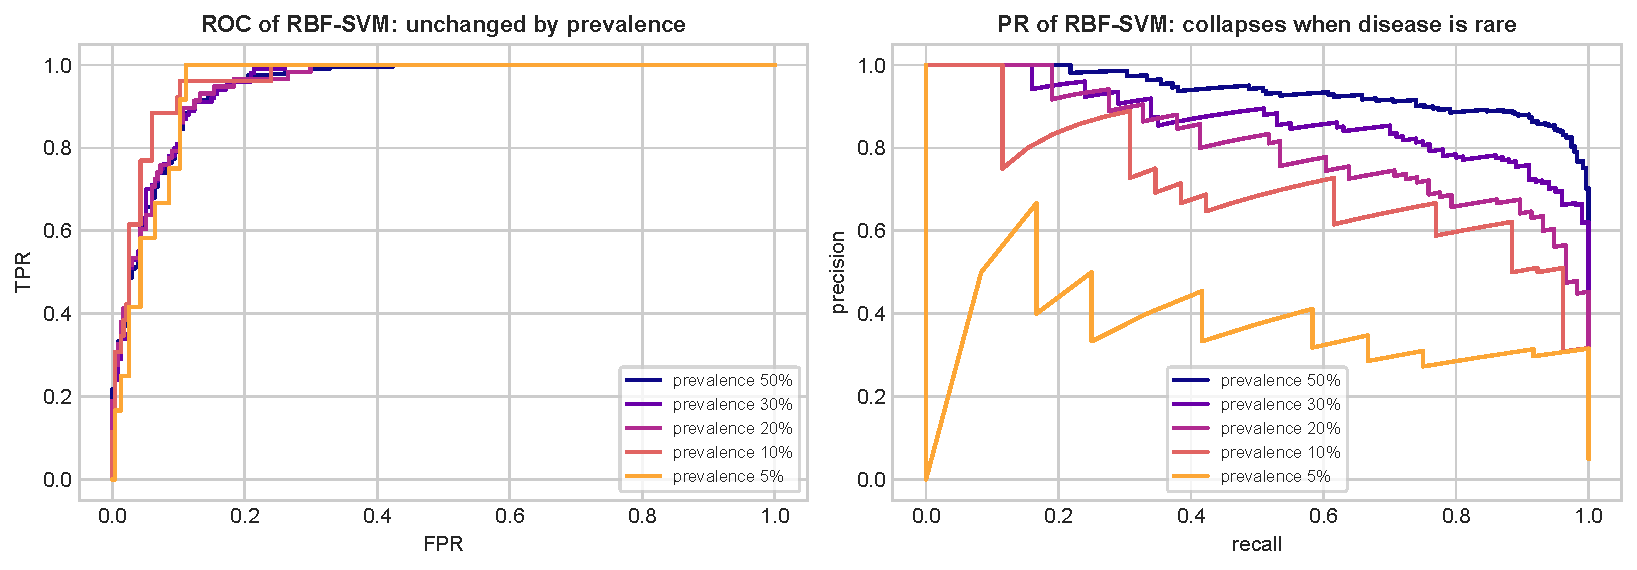
\includegraphics[width=\linewidth]{fig_prevalence}
  \caption{Même classifieur (SVM RBF), mêmes scores~: les courbes ROC sont invariantes à la prévalence de la classe
           positive, les courbes précision--rappel s'effondrent quand la maladie devient rare.}
  \label{fig:prevalence}
\end{figure}

\subsection{Robustesse des modèles classiques au bruit d'étiquetage}
Avec 5\,\% des étiquettes normales d'entraînement inversées (table~\ref{tab:noise5}), les modèles de référence perdent
environ un point d'exactitude et 2 à 4 points de spécificité, tandis que leur AUC ROC est inchangée~; le F1, dominé par
la classe majoritaire, bouge à peine. Le balayage de la figure~\ref{fig:noise_classical} révèle le mécanisme. Jusqu'à
40\,\% d'étiquettes minoritaires inversées, la spécificité des modèles de référence s'effondre d'environ 0,6 à 0,19--0,32
et leur exactitude tombe à 0,70--0,74, alors que l'AUC ROC reste entre 0,92 et 0,95~: \textbf{le bruit asymétrique
déplace le seuil de décision plutôt que le classement}. Les modèles ordonnent toujours correctement les patients, mais
ils ont appris une prévalence de pneumonie surestimée. De façon cohérente, \textbf{une régularisation plus forte n'aide
pas}~: les variantes régularisées sont moins bonnes que les modèles de référence à tous les niveaux de bruit, car un
modèle plus contraint s'appuie davantage sur l'a priori de classe (corrompu). À l'inverse, re-choisir simplement le
seuil sur le petit ensemble de validation propre maintient l'exactitude des trois modèles entre 0,85 et 0,89 de 0 à
40\,\% de bruit. Ce remède suppose un sous-ensemble étiqueté de confiance et n'indique pas \emph{quelles} étiquettes
d'entraînement sont fausses.

\begin{table}[t]
\centering
\small
\caption{Robustesse à l'inversion de 5\,\% des étiquettes d'entraînement de la classe minoritaire (normale). \emph{référence}~: hyperparamètres choisis sur la validation~; \emph{robuste}~: régularisation plus forte~; \emph{recalibrée}~: modèle de référence dont le seuil de décision est re-choisi sur la validation propre. Propre~: une exécution~; bruité~: moyenne$\pm$écart-type sur 10 tirages. $\Delta$ = bruité $-$ propre (le test est toujours propre).}
\label{tab:noise5}
\begin{adjustbox}{max width=\textwidth}
\begin{tabular}{llccccccccc}
\toprule
Modèle & Config. & Acc. propre & Acc. bruité & $\Delta$Acc. & Spéc. propre & Spéc. bruité & $\Delta$Spéc. & AUC propre & AUC bruité & $\Delta$AUC \\
\midrule
Gradient boosting & référence & 0,830 & 0,825$\pm$0,005 & -0,006 & 0,594 & 0,560$\pm$0,013 & -0,034 & 0,938 & 0,940$\pm$0,003 & +0,002 \\
Gradient boosting & recalibrée & 0,838 & 0,867$\pm$0,011 & +0,029 & 0,624 & 0,721$\pm$0,056 & +0,097 & 0,938 & 0,940$\pm$0,003 & +0,002 \\
Gradient boosting & robuste & 0,824 & 0,806$\pm$0,006 & -0,018 & 0,573 & 0,521$\pm$0,016 & -0,052 & 0,932 & 0,930$\pm$0,002 & -0,001 \\
SVM RBF & référence & 0,857 & 0,849$\pm$0,004 & -0,008 & 0,632 & 0,609$\pm$0,011 & -0,023 & 0,947 & 0,947$\pm$0,002 & -0,001 \\
SVM RBF & recalibrée & 0,872 & 0,875$\pm$0,016 & +0,004 & 0,671 & 0,692$\pm$0,055 & +0,021 & 0,947 & 0,947$\pm$0,002 & -0,001 \\
SVM RBF & robuste & 0,841 & 0,833$\pm$0,004 & -0,008 & 0,598 & 0,570$\pm$0,011 & -0,029 & 0,946 & 0,946$\pm$0,001 & -0,000 \\
LogReg & référence & 0,837 & 0,826$\pm$0,003 & -0,011 & 0,590 & 0,550$\pm$0,008 & -0,039 & 0,923 & 0,923$\pm$0,001 & -0,000 \\
LogReg & recalibrée & 0,865 & 0,869$\pm$0,004 & +0,003 & 0,722 & 0,725$\pm$0,015 & +0,003 & 0,923 & 0,923$\pm$0,001 & -0,000 \\
LogReg & robuste & 0,822 & 0,802$\pm$0,002 & -0,020 & 0,551 & 0,494$\pm$0,004 & -0,058 & 0,920 & 0,919$\pm$0,000 & -0,000 \\
\bottomrule
\end{tabular}
\end{adjustbox}
\end{table}


\begin{figure}[t]
  \centering
  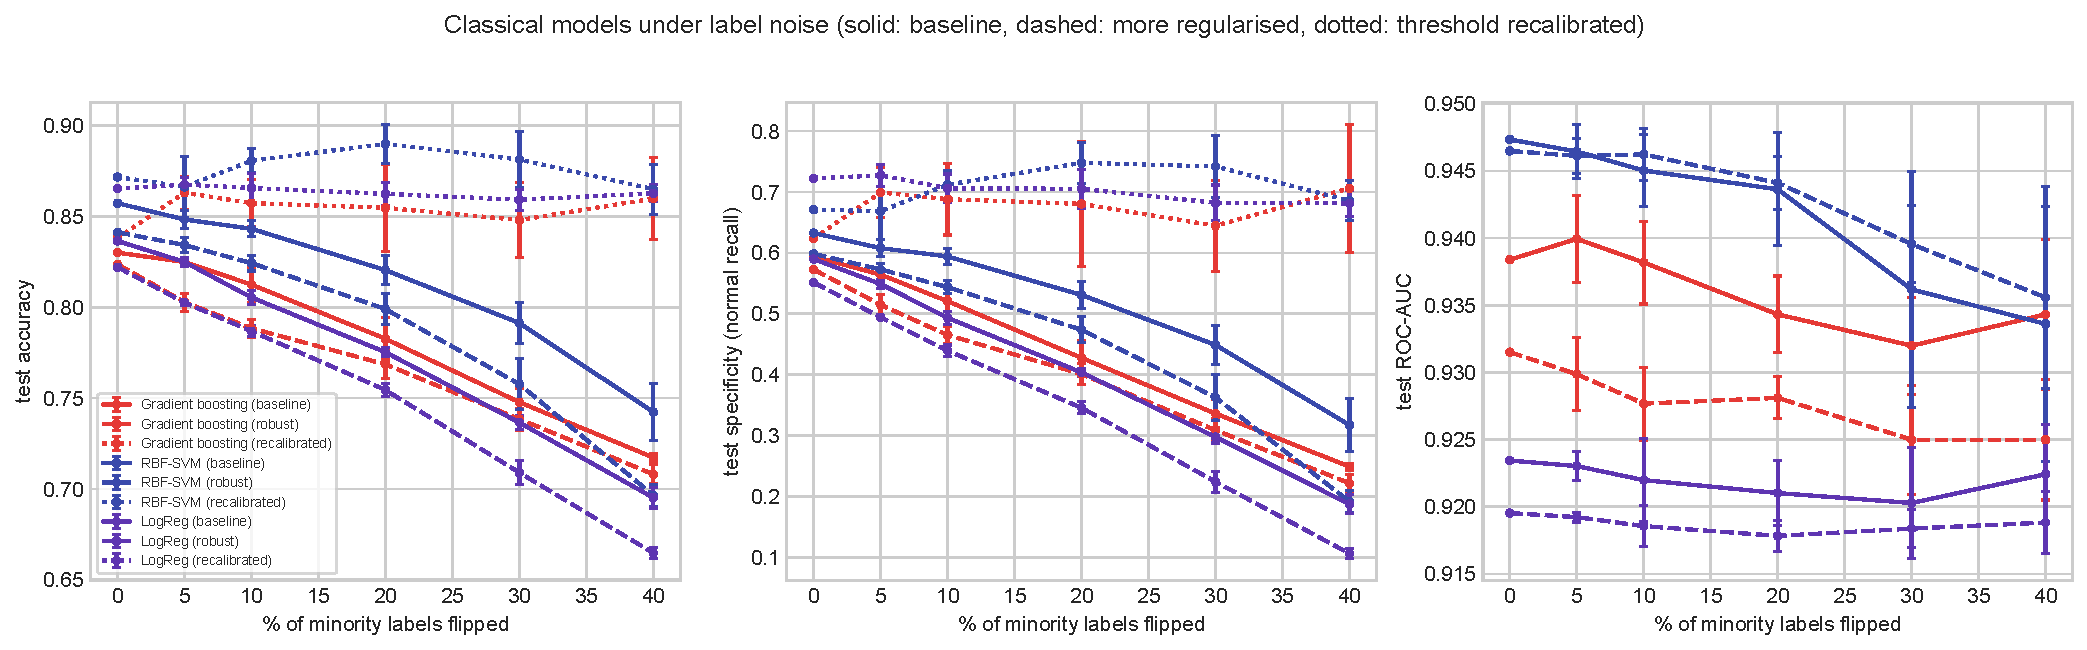
\includegraphics[width=\linewidth]{fig_noise_sweep_classical}
  \caption{Exactitude, spécificité et AUC ROC en test des trois modèles classiques retenus lorsqu'une fraction
           croissante des étiquettes d'entraînement minoritaires (normales) est inversée (moyenne\,$\pm$\,écart-type sur
           5 tirages). Trait plein~: référence~; tirets~: régularisation plus forte~; pointillés~: référence avec le seuil
           de décision recalibré sur la validation propre.}
  \label{fig:noise_classical}
\end{figure}

\subsection{CNN évidentiel contre CNN softmax}
La table~\ref{tab:edl} et la figure~\ref{fig:noise_all} comparent les deux CNN au meilleur modèle classique. Au seuil
par défaut de 0,5, les deux CNN sont \emph{moins} exacts que le SVM RBF (0,779\,$\pm$\,0,067 pour le softmax et
0,761\,$\pm$\,0,084 pour l'EDL sur étiquettes propres, contre 0,857) et varient fortement d'une graine à l'autre, bien
qu'ils classent aussi bien les patients (AUC ROC 0,94 à 0,96). De petits CNN sur-apprennent la prévalence
d'entraînement encore plus que les modèles classiques~: leur spécificité est faible et instable. Une fois le seuil
re-choisi sur la validation propre, tous les modèles convergent vers une exactitude de 0,86 à 0,87 sur étiquettes
propres. À architecture égale, la tête évidentielle n'améliore ni ne dégrade la classification~: à chaque niveau de
bruit, les exactitudes moyennes des modèles softmax et EDL diffèrent d'au plus 0,03, bien en deçà de leur variabilité
entre graines (figure~\ref{fig:noise_all}). Le modèle évidentiel est en revanche systématiquement \textbf{mieux
calibré}~: son erreur de calibration attendue est plus faible aux six niveaux de bruit, et l'écart se creuse sous bruit
(0,144 contre 0,174 sur étiquettes propres, 0,126 contre 0,206 à 20\,\% et 0,187 contre 0,241 à 40\,\% d'étiquettes
inversées). Le terme KL, qui retire l'évidence non justifiée par les étiquettes, empêche la sur-confiance que l'entropie
croisée induit sur les exemples contradictoires.

\begin{table}[t]
\centering
\small
\caption{Performances en test (propre) après entraînement avec des étiquettes minoritaires inversées (moyenne$\pm$écart-type sur les seeds~: 5 pour le modèle classique, 3 pour les CNN). \emph{recal.}~: seuil de décision re-choisi sur la validation propre. ECE~: Expected Calibration Error (plus faible = meilleure).}
\label{tab:edl}
\begin{adjustbox}{max width=\textwidth}
\begin{tabular}{llcccccc}
\toprule
Bruit & Modèle & Acc. & Spéc. & ROC-AUC & Acc. (recal.) & Spéc. (recal.) & ECE \\
\midrule
0\% & SVM RBF (classique) & 0,857 & 0,632 & 0,947 & 0,872 & 0,671 & n.d. \\
0\% & CNN softmax & 0,779$\pm$0,067 & 0,419$\pm$0,187 & 0,946$\pm$0,001 & 0,869$\pm$0,010 & 0,682$\pm$0,012 & 0,174$\pm$0,080 \\
0\% & CNN EDL & 0,761$\pm$0,084 & 0,377$\pm$0,250 & 0,940$\pm$0,014 & 0,860$\pm$0,011 & 0,661$\pm$0,040 & 0,144$\pm$0,075 \\
5\% & SVM RBF (classique) & 0,848$\pm$0,005 & 0,608$\pm$0,014 & 0,946$\pm$0,002 & 0,866$\pm$0,017 & 0,668$\pm$0,060 & n.d. \\
5\% & CNN softmax & 0,810$\pm$0,055 & 0,504$\pm$0,158 & 0,946$\pm$0,011 & 0,856$\pm$0,025 & 0,634$\pm$0,073 & 0,129$\pm$0,054 \\
5\% & CNN EDL & 0,798$\pm$0,096 & 0,486$\pm$0,298 & 0,950$\pm$0,025 & 0,862$\pm$0,038 & 0,660$\pm$0,114 & 0,128$\pm$0,045 \\
20\% & SVM RBF (classique) & 0,821$\pm$0,008 & 0,531$\pm$0,022 & 0,944$\pm$0,004 & 0,890$\pm$0,011 & 0,748$\pm$0,034 & n.d. \\
20\% & CNN softmax & 0,722$\pm$0,049 & 0,259$\pm$0,129 & 0,950$\pm$0,013 & 0,855$\pm$0,012 & 0,658$\pm$0,045 & 0,206$\pm$0,058 \\
20\% & CNN EDL & 0,755$\pm$0,053 & 0,349$\pm$0,146 & 0,949$\pm$0,021 & 0,863$\pm$0,037 & 0,681$\pm$0,126 & 0,126$\pm$0,050 \\
\bottomrule
\end{tabular}
\end{adjustbox}
\end{table}


\begin{figure}[t]
  \centering
  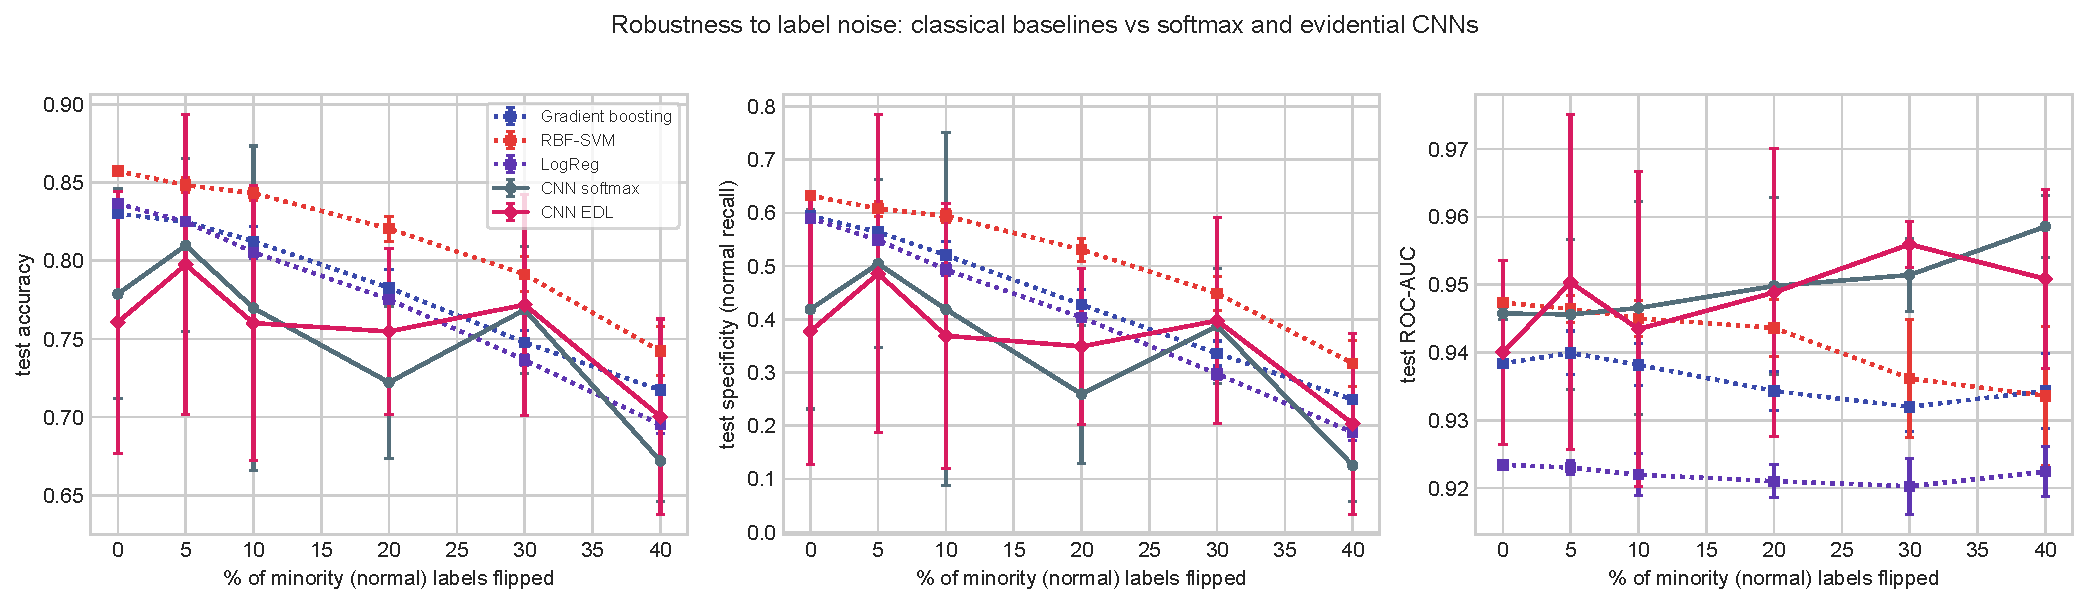
\includegraphics[width=\linewidth]{fig_noise_sweep_all}
  \caption{Modèles classiques de référence (pointillés, 5 tirages) contre CNN softmax et évidentiel (traits pleins,
           3 graines) sous un bruit croissant sur les étiquettes minoritaires, au seuil de décision par défaut.}
  \label{fig:noise_all}
\end{figure}

\subsection{À quoi sert l'incertitude évidentielle~?}
La table~\ref{tab:uncertainty} et la figure~\ref{fig:uncertainty} évaluent l'incertitude elle-même.
\emph{Renvoi des cas douteux.} Les deux scores d'incertitude séparent les prédictions erronées des prédictions correctes
avec une AUROC d'environ 0,80 à 0,84, sans vainqueur constant. Pour la graine montrée à la
figure~\ref{fig:uncertainty} (gauche), le modèle évidentiel conserve une meilleure exactitude à presque tous les taux de
renvoi, en particulier lorsqu'il est entraîné avec 20\,\% de bruit~; avec trois graines, cette observation reste à
confirmer sur davantage d'exécutions.
\emph{Étiquettes d'entraînement inversées.} Avec 20\,\% des étiquettes normales inversées, l'incertitude place les
images inversées au-dessus des autres avec une AUROC de 0,88 pour les deux modèles, et le désaccord entre la prédiction
évidentielle et l'étiquette fournie atteint 0,924\,$\pm$\,0,060 (0,899 pour le softmax). La figure~\ref{fig:uncertainty}
(droite) nuance ce résultat~: les images inversées reçoivent un $u$ élevé \emph{parce que ce sont des radiographies
normales}~; c'est toute la classe contestée qui devient incertaine, et non chaque exemple inversé qui se distingue de
ses pairs normaux. Le signal est donc utile pour orienter la ré-annotation vers la classe touchée plutôt que pour
désigner chaque erreur.
\emph{Images hors distribution.} Le $u$ évidentiel ne surpasse pas systématiquement l'entropie softmax~: il est moins
bon sur les échographies (0,763 contre 0,814 sur étiquettes propres), comparable sur les scanners, et meilleur sur les
scanners seulement après un entraînement sur étiquettes bruitées (0,847 contre 0,795). La figure~\ref{fig:dirichlet}
illustre ce qu'apporte la sortie de Dirichlet~: sur l'image de test où le modèle évidentiel est le plus indécis, le
softmax prédit une pneumonie avec une probabilité de 0,83 tandis que l'EDL renvoie une loi symétrique
$\mathrm{Beta}(2{,}9~;~2{,}9)$ avec $u=0{,}35$~; sur une échographie, le softmax répond 0,56 et l'EDL une densité plate
avec $u=0{,}46$, c'est-à-dire «~je ne sais pas~» plutôt que «~pneumonie un peu plus probable~».

\begin{table}[t]
\centering
\small
\caption{AUROC des scores d'incertitude (moyenne$\pm$écart-type sur 3 graines) pour détecter les images de test mal classées, les images hors distribution (échographies BreastMNIST, scanners OrganCMNIST) et les étiquettes d'entraînement inversées. \emph{Désacc.}~: $1-\hat p(\text{étiquette fournie})$.}
\label{tab:uncertainty}
\begin{adjustbox}{max width=\textwidth}
\begin{tabular}{llccccc}
\toprule
Bruit (entraîn.) & Modèle (incertitude) & Erreurs & OOD échographie & OOD scanner & Inversées ($u$) & Inversées (désacc.) \\
\midrule
0\% & CNN EDL ($u=K/S$) & 0,830$\pm$0,006 & 0,763$\pm$0,029 & 0,650$\pm$0,213 & -- & -- \\
0\% & CNN softmax (entropie) & 0,822$\pm$0,016 & 0,814$\pm$0,009 & 0,675$\pm$0,065 & -- & -- \\
20\% & CNN EDL ($u=K/S$) & 0,801$\pm$0,030 & 0,753$\pm$0,110 & 0,847$\pm$0,026 & 0,882$\pm$0,012 & 0,924$\pm$0,060 \\
20\% & CNN softmax (entropie) & 0,836$\pm$0,051 & 0,829$\pm$0,043 & 0,795$\pm$0,031 & 0,885$\pm$0,017 & 0,899$\pm$0,058 \\
\bottomrule
\end{tabular}
\end{adjustbox}
\end{table}


\begin{figure}[t]
  \centering
  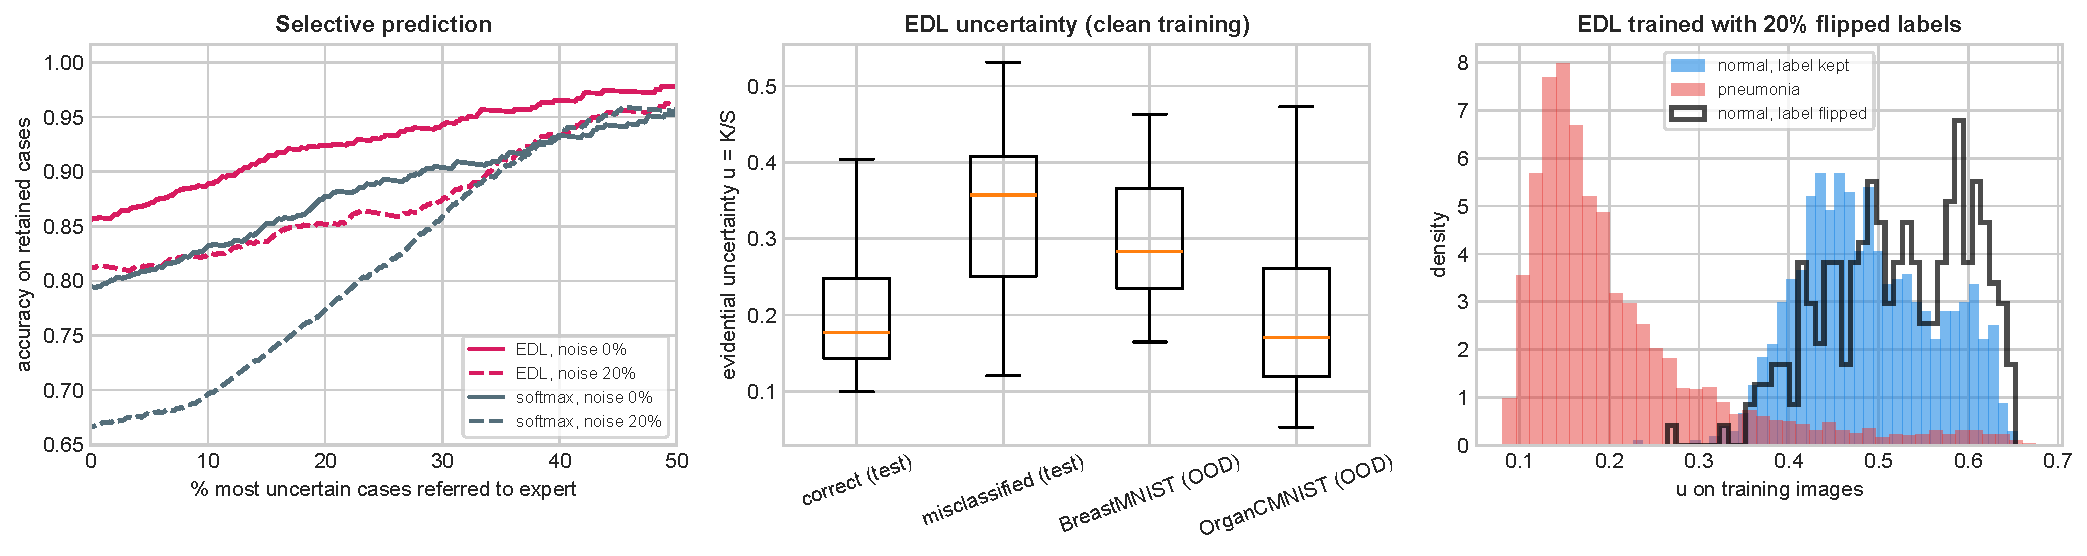
\includegraphics[width=\linewidth]{fig_uncertainty}
  \caption{Gauche~: prédiction sélective, c'est-à-dire l'exactitude sur les cas conservés lorsque les images de test les
           plus incertaines sont renvoyées à un expert (graine 0). Centre~: incertitude évidentielle des images
           correctement classées, mal classées et hors distribution (entraînement propre). Droite~: incertitude
           évidentielle sur les images d'entraînement après inversion de 20\,\% des étiquettes normales.}
  \label{fig:uncertainty}
\end{figure}

\begin{figure}[t]
  \centering
  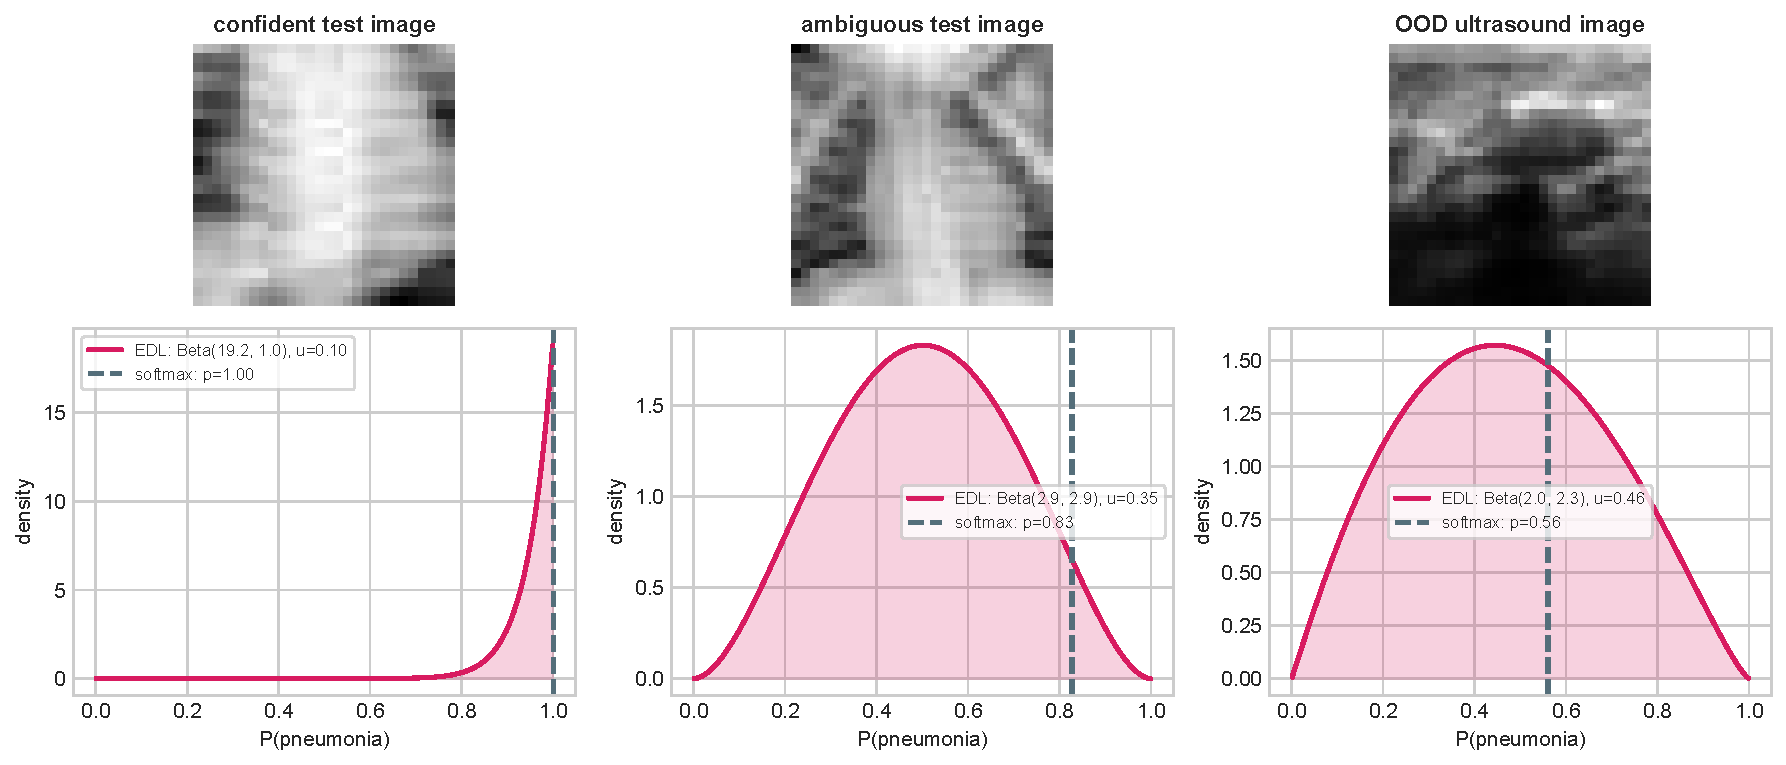
\includegraphics[width=0.92\linewidth]{fig_dirichlet}
  \caption{Sorties de Dirichlet (ici Beta, $K=2$) du CNN évidentiel pour une image de test certaine, l'image de test sur
           laquelle il est le plus indécis et une échographie hors distribution, face à la prédiction ponctuelle du CNN
           softmax de même architecture.}
  \label{fig:dirichlet}
\end{figure}

% ======================================================================
\section{Discussion et limites}
% ======================================================================
Nos expériences séparent deux effets souvent confondus sous le terme de «~robustesse au bruit d'étiquetage~». Pour un
bruit conditionnel à la classe minoritaire, l'effet dominant est un \emph{décalage d'a priori}~: l'a priori de classe
appris est surestimé, le classement est préservé, et le dommage est réparé en recalibrant un unique seuil sur des
données de confiance. La régularisation, elle, s'attaque à la \emph{mémorisation}, qui n'est pas le mode de défaillance
ici et aggrave même le décalage d'a priori. L'apprentissage évidentiel apporte un troisième bénéfice, orthogonal~: une
confiance calibrée et une masse d'ignorance explicite, qui rendent les défaillances du modèle plus visibles plutôt que
moins fréquentes.

Ces conclusions ont des limites. Les images font $28\times28$ pixels, ce qui avantage les modèles classiques et limite
les CNN~; le bruit est synthétique et conditionnel à la classe, alors que les vraies erreurs d'annotation dépendent de
l'image~; un seul jeu de données, présentant un net décalage de prévalence entre entraînement et test, est utilisé~; les
CNN ont été entraînés avec trois graines sur CPU et présentent une forte variance~; enfin, la recalibration du seuil
suppose un petit ensemble de validation propre, ressource réaliste mais non gratuite en pratique clinique. La détection
hors distribution n'a été évaluée que sur deux autres modalités de MedMNIST.

% ======================================================================
\section{Conclusion et perspectives}
% ======================================================================
Sur PneumoniaMNIST, l'inversion d'étiquettes de la classe minoritaire déplace surtout le seuil de décision des
classifieurs classiques en laissant leur classement intact. Une régularisation plus forte n'aide pas, mais recalibrer le
seuil sur un petit ensemble propre neutralise l'essentiel du dommage. Un CNN évidentiel classe aussi bien que son jumeau
softmax, est mieux calibré sous bruit et exprime explicitement son ignorance, même si son incertitude n'est pas un
détecteur fiable d'images hors distribution dans notre cadre. Vers une chaîne évidentielle complète, nous prévoyons
(i)~d'utiliser l'incertitude évidentielle pour repondérer ou ré-étiqueter les exemples d'entraînement suspects plutôt que
de seulement la rapporter~; (ii)~d'exploiter plusieurs annotateurs et les étiquettes explicitement \emph{incertaines} de
CheXpert~\cite{irvin2019chexpert} en pleine résolution, où les modèles profonds ont un réel avantage~; (iii)~de combiner
l'EDL avec une correction du décalage d'a priori et une calibration a posteriori~; et (iv)~de la comparer aux ensembles
profonds et au dropout Monte-Carlo~\cite{lakshminarayanan2017simple,gal2016dropout} à budget de calcul égal.

\section*{Remerciements}
Ce travail a été réalisé dans le cadre du Travail Pratique~4 du cours d'apprentissage automatique du Département de
Génie Informatique de l'École Nationale Supérieure Polytechnique de Yaoundé (ENSPY), Université de Yaoundé~I, sous la
supervision du Dr~Louis Fippo Fitime, de Claude Tinku et de Kerolle Sonfack.

\section*{Disponibilité du code et des données}
PneumoniaMNIST, OrganCMNIST et BreastMNIST sont disponibles publiquement via MedMNIST~\cite{yang2023medmnist}. Les quatre
notebooks, le module partagé et la configuration MLflow qui produisent chaque nombre, table et figure de ce rapport sont
fournis avec celui-ci~; tous les hyperparamètres ont été choisis sur la partition de validation et toutes les graines
aléatoires sont fixées.

\bibliographystyle{plainnat}
\bibliography{references}

% ======================================================================
\appendix
\section{Figures complémentaires (phases I et II)}
% ======================================================================
\begin{figure}[h]
  \centering
  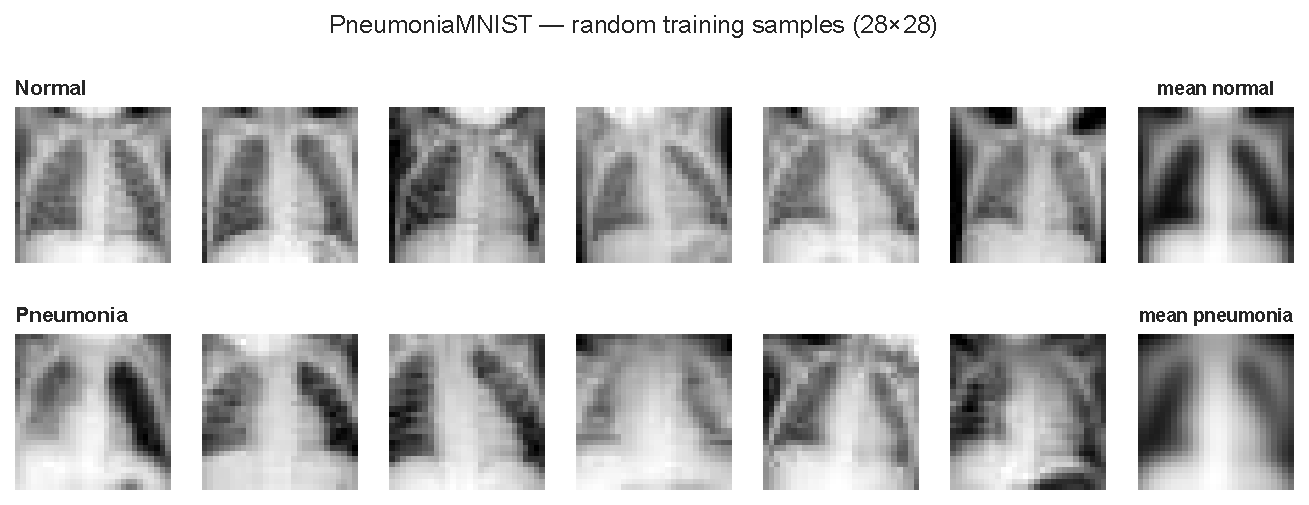
\includegraphics[width=0.85\linewidth]{fig_samples}
  \caption{Images d'entraînement de PneumoniaMNIST tirées au hasard et images moyennes par classe.}
  \label{fig:samples}
\end{figure}

\begin{figure}[h]
  \centering
  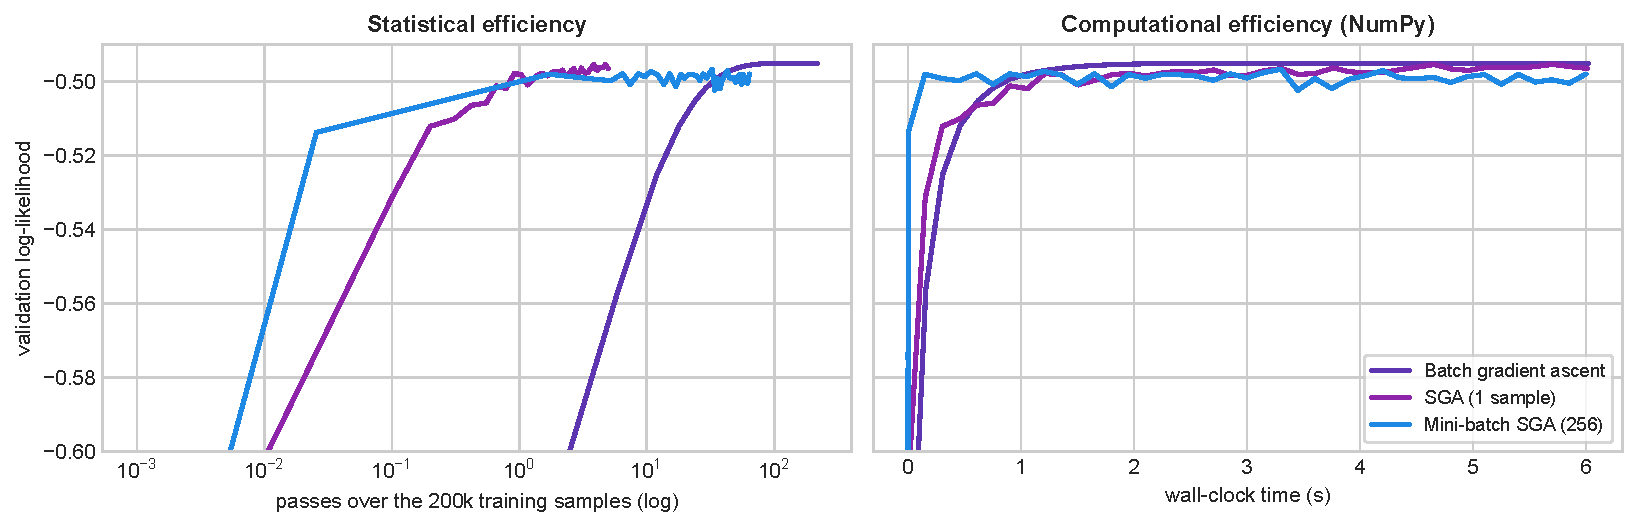
\includegraphics[width=\linewidth]{fig_sga_scaling}
  \caption{Régression logistique sur 200\,000 exemples synthétiques. Gauche~: log-vraisemblance de validation en fonction
           du nombre de passes sur les données~; les mises à jour stochastiques n'ont besoin que d'une fraction de passe,
           la montée de gradient par lot de dizaines de passes. Droite~: temps réel~; la boucle Python exemple par exemple
           paie le coût de l'interpréteur, le SGA par mini-lots cumule les deux avantages.}
  \label{fig:sga}
\end{figure}

\begin{figure}[h]
  \centering
  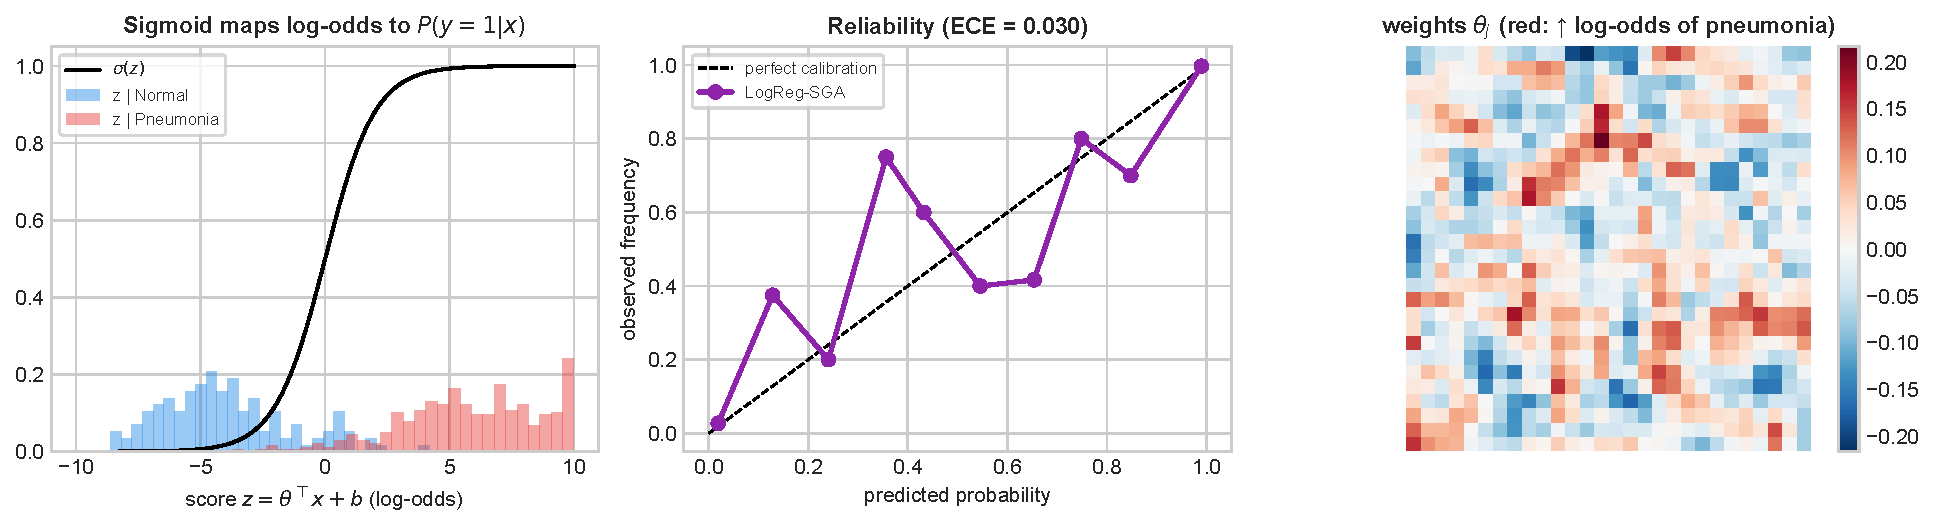
\includegraphics[width=\linewidth]{fig_logreg_proba}
  \caption{Lecture probabiliste de la sigmoïde (régression logistique SGA, validation)~: log-cotes par classe, diagramme
           de fiabilité et poids $\theta_j$ affichés comme une image.}
  \label{fig:logreg}
\end{figure}

\begin{figure}[h]
  \centering
  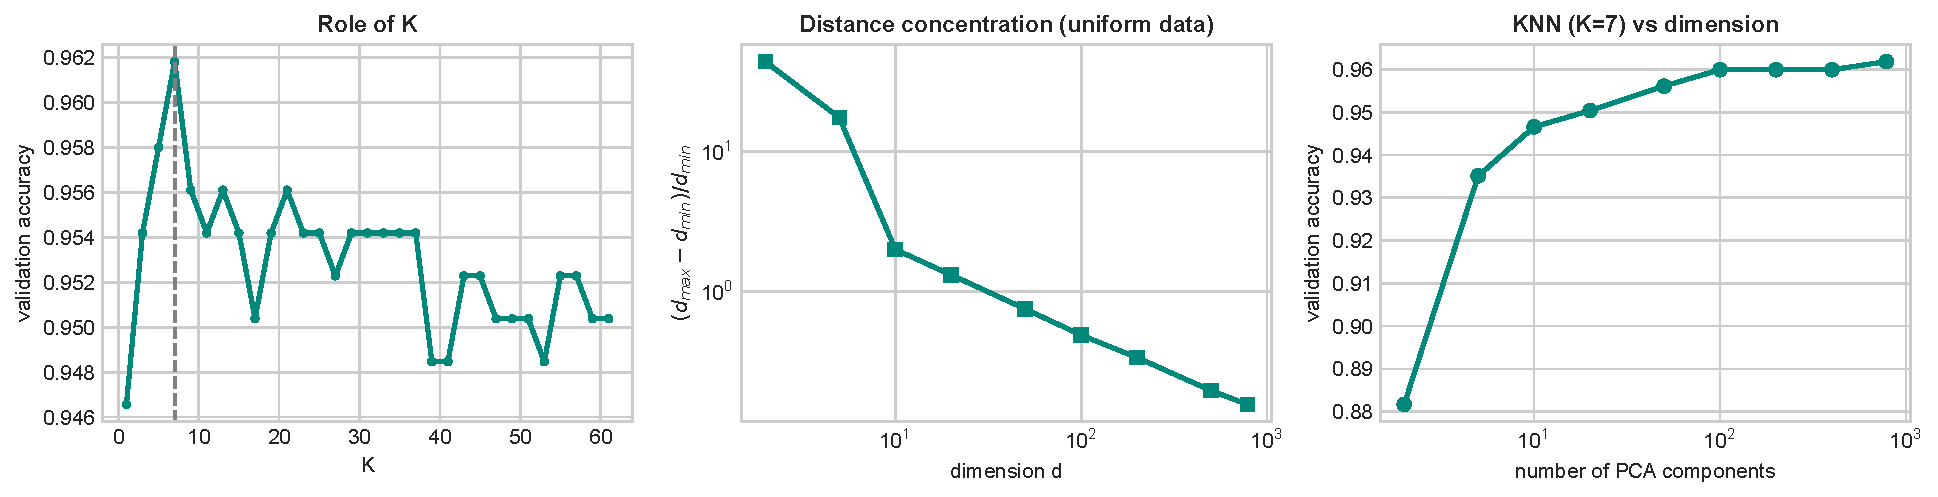
\includegraphics[width=\linewidth]{fig_knn}
  \caption{$K$ plus proches voisins~: exactitude de validation en fonction de $K$~; concentration des distances sur des
           données uniformes~; exactitude en fonction du nombre de composantes ACP. Les radiographies vivent sur une
           variété de faible dimension, si bien que KNN se dégrade bien moins que ne le suggère le cas uniforme.}
  \label{fig:knn}
\end{figure}

\begin{figure}[h]
  \centering
  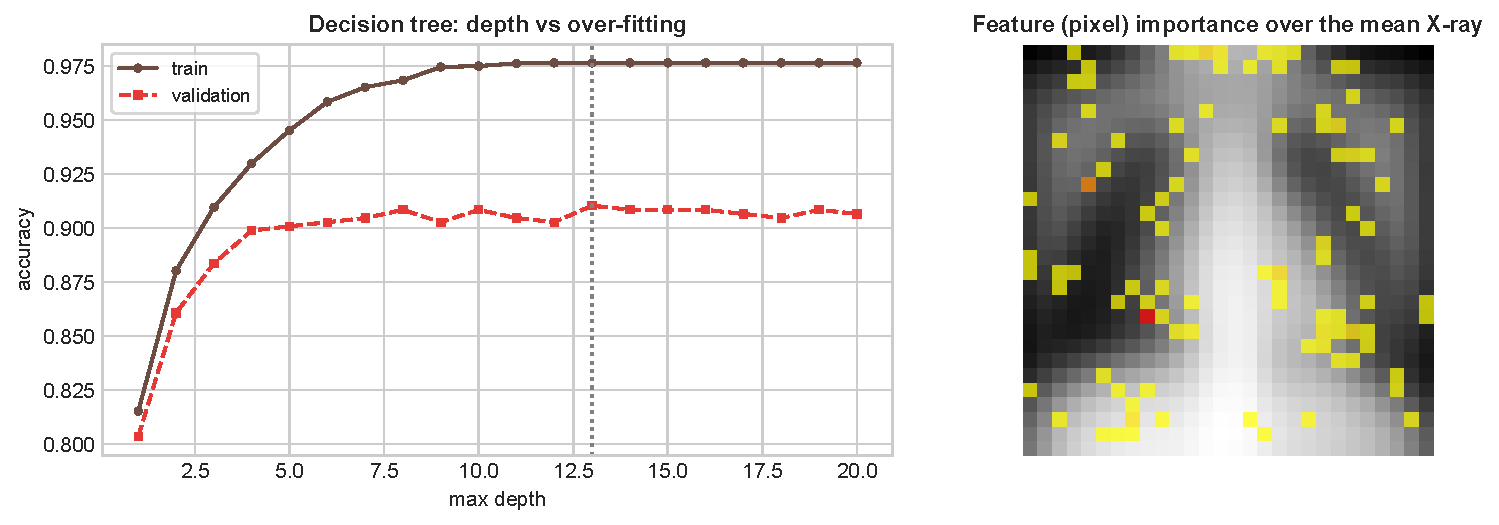
\includegraphics[width=0.9\linewidth]{fig_tree}\\[4pt]
  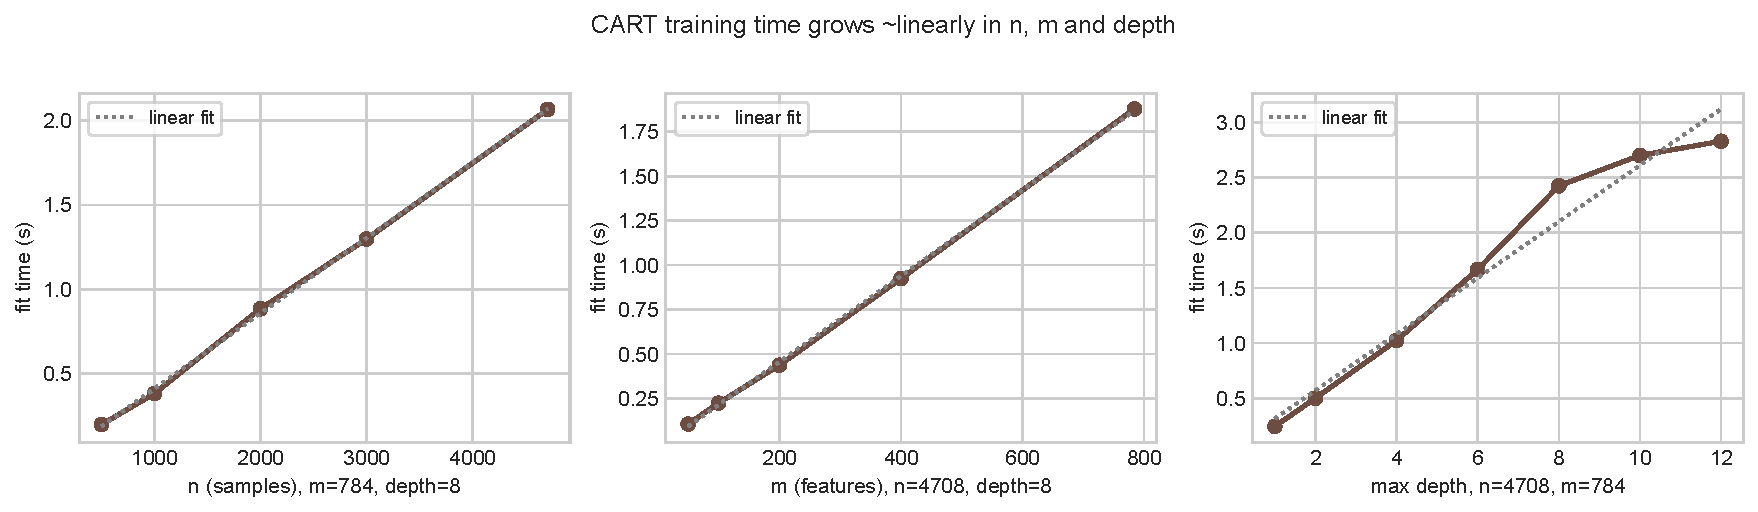
\includegraphics[width=\linewidth]{fig_tree_complexity}
  \caption{Arbre de décision. Haut~: choix de la profondeur et importance des pixels (diminution moyenne de l'impureté)
           sur la radiographie moyenne. Bas~: le temps d'apprentissage de CART croît linéairement en $n$, $m$ et en
           profondeur, soit $O(n\cdot m\cdot\text{profondeur})$ à un facteur logarithmique près.}
  \label{fig:tree}
\end{figure}

\begin{figure}[h]
  \centering
  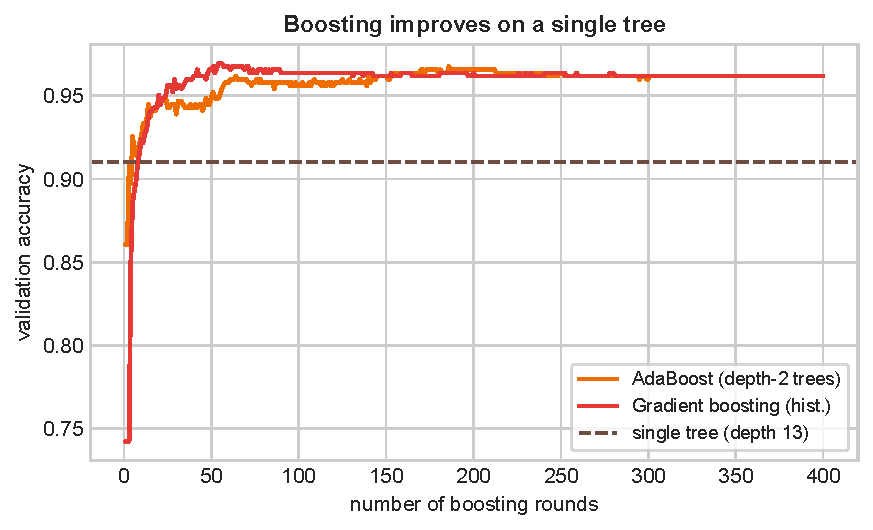
\includegraphics[width=0.6\linewidth]{fig_boosting}
  \caption{Exactitude de validation en fonction du nombre d'itérations de boosting.}
  \label{fig:boosting}
\end{figure}

\begin{figure}[h]
  \centering
  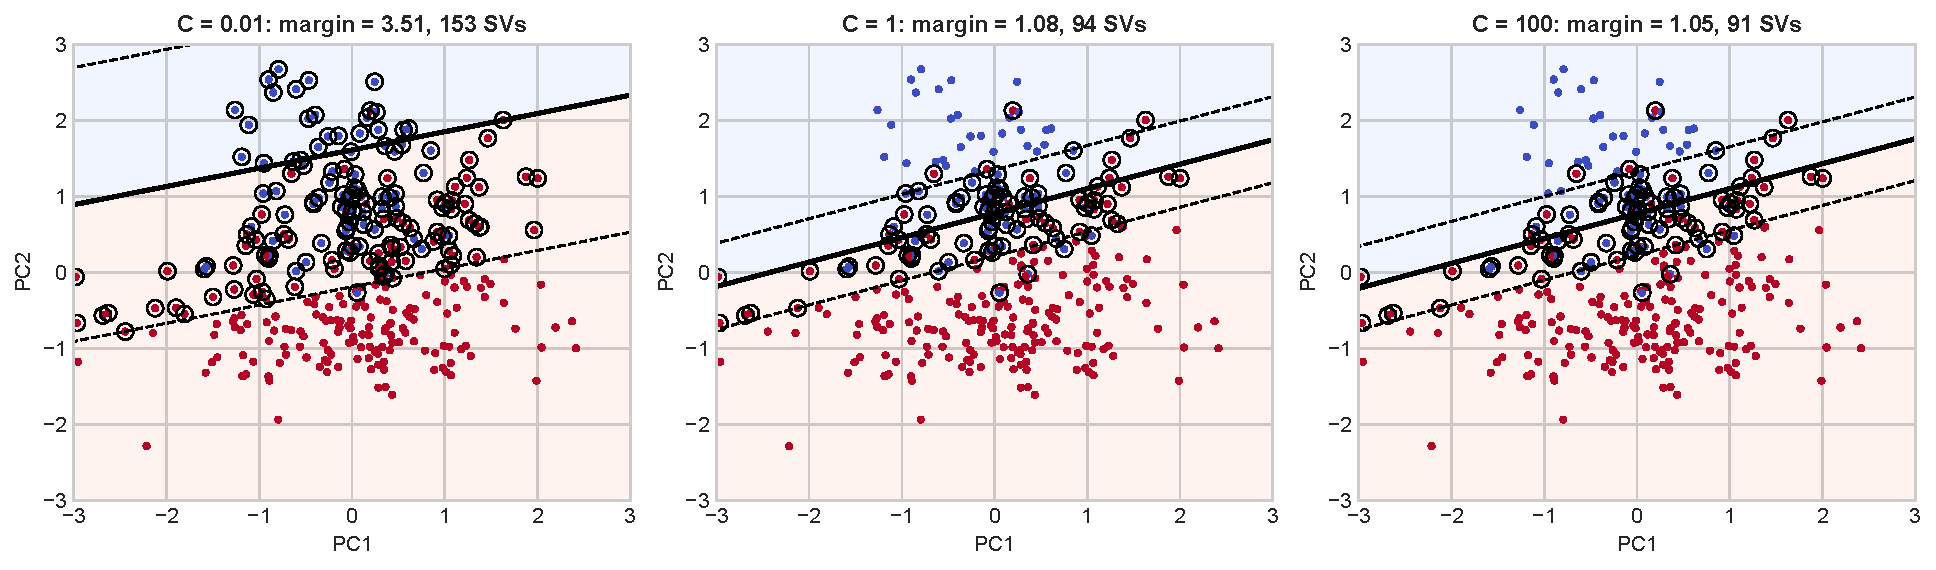
\includegraphics[width=\linewidth]{fig_svm_margin}\\[4pt]
  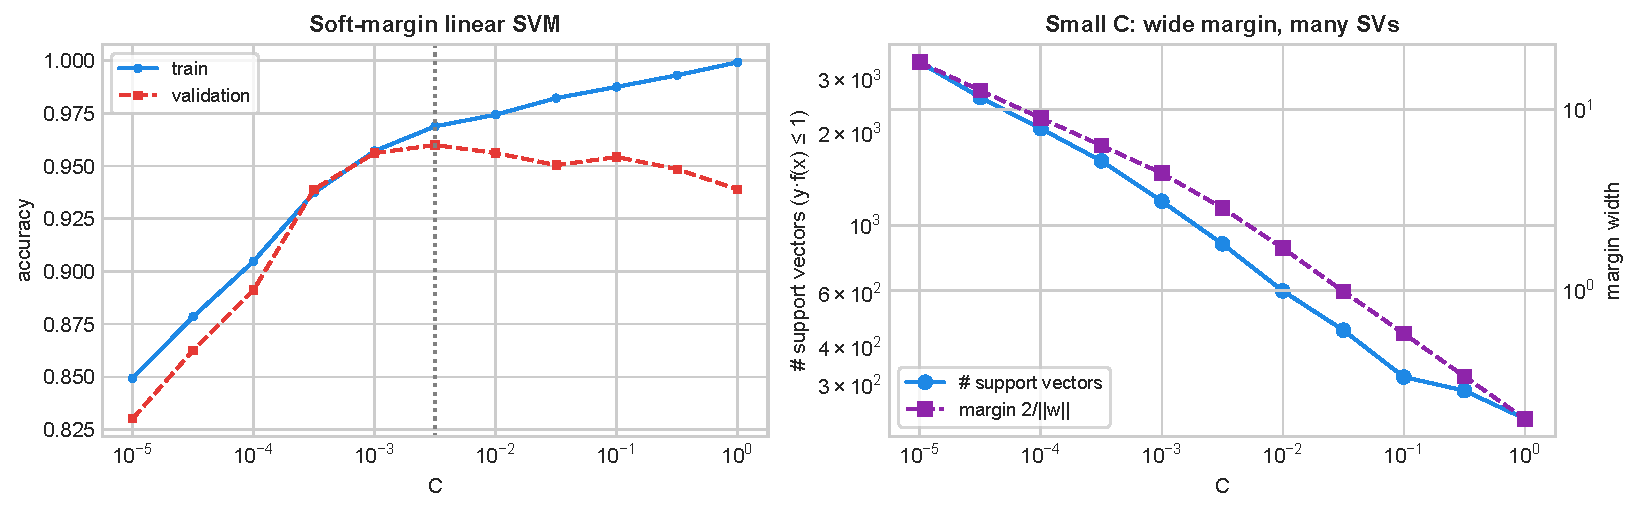
\includegraphics[width=\linewidth]{fig_svm_C}
  \caption{Machines à vecteurs de support. Haut~: SVM linéaire sur une projection 2D pour trois valeurs de $C$ (points
           cerclés~: vecteurs supports~; tirets~: marge). Bas~: sur les 784 pixels, un petit $C$ donne une marge large et
           beaucoup de vecteurs supports (forte régularisation), un grand $C$ une marge étroite qui colle à
           l'entraînement.}
  \label{fig:svm}
\end{figure}

\begin{figure}[h]
  \centering
  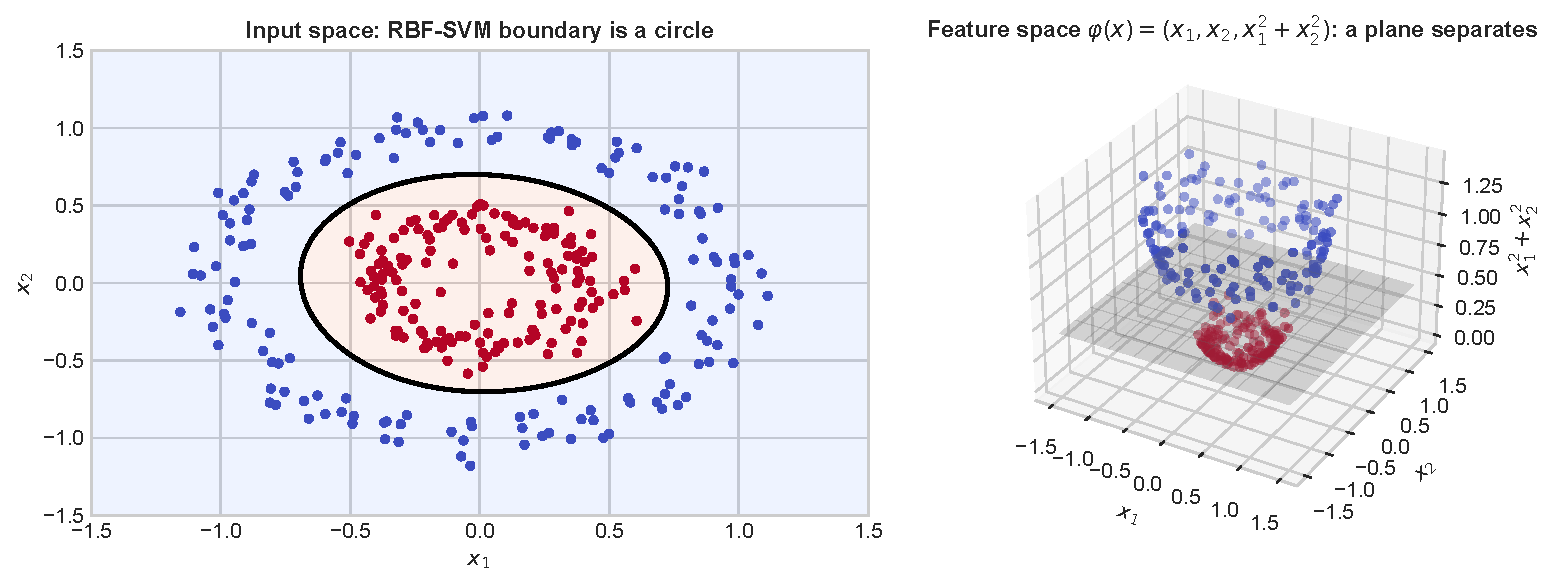
\includegraphics[width=0.62\linewidth]{fig_kernel_trick}\hfill
  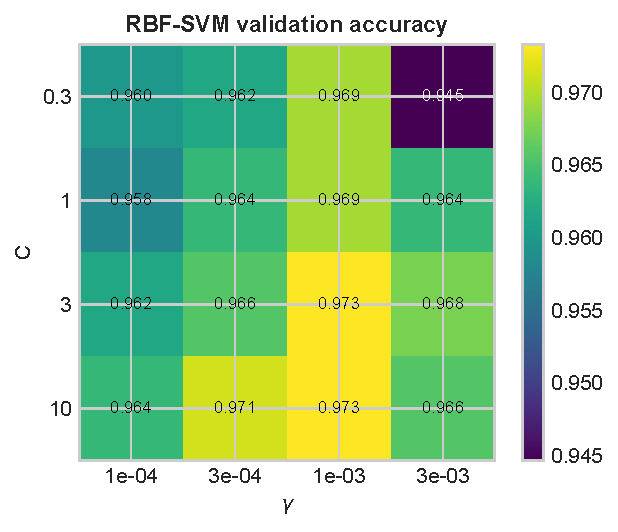
\includegraphics[width=0.34\linewidth]{fig_svm_rbf_grid}
  \caption{Gauche~: l'astuce du noyau, où des classes concentriques deviennent linéairement séparables après la
           projection explicite $\varphi(x)=(x_1,x_2,x_1^2+x_2^2)$~; le noyau RBF le fait implicitement dans un espace de
           dimension infinie. Droite~: exactitude de validation du SVM RBF selon $(C,\gamma)$.}
  \label{fig:kernel}
\end{figure}

\begin{figure}[h]
  \centering
  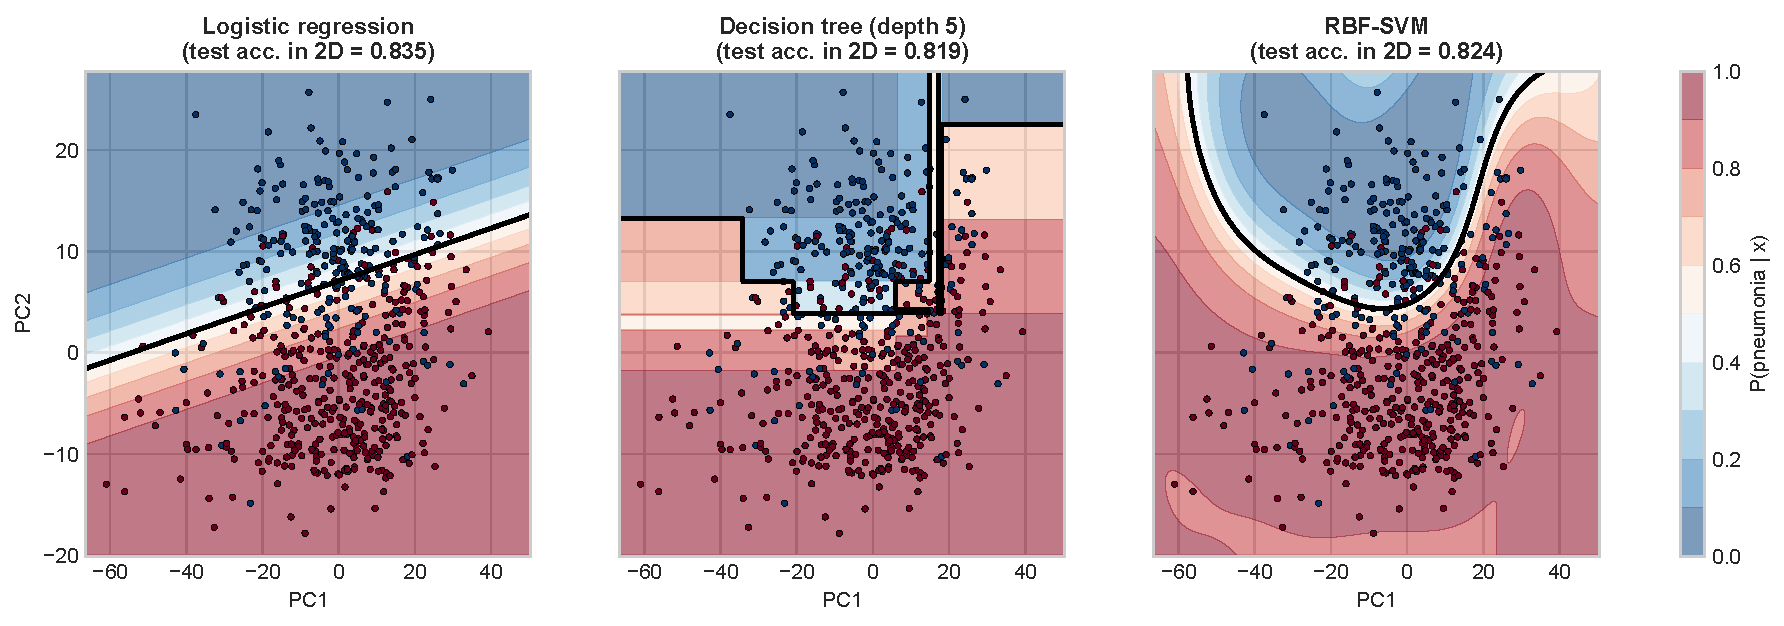
\includegraphics[width=\linewidth]{fig_boundaries}
  \caption{Frontières de décision ($P=0{,}5$, en noir) et probabilités prédites sur les deux premières composantes
           principales~: régression logistique (linéaire), arbre de décision (aligné sur les axes, constant par morceaux)
           et SVM RBF (lisse et courbe).}
  \label{fig:boundaries}
\end{figure}

\end{document}
